\textbf{Sliding mode control (SMC)} is a well-estabilished method for control of nonlinear systems, and is characterized (like Feedback linearization) by solid theoretical foundations. An interesting feature of SMC is the robustness against \textbf{imprecise knowledge of the plant to control}. \\
\textbf{General Approach}:
\begin{enumerate}
    \item A \textbf{sliding surface} is defined. This surface is a subset of the state domain where the system can have \textbf{good properties}.
    \item A feedback law is designed in order to bring the plant trajectory towards the sliding surface and once there, to stay close to this surface. 
\end{enumerate}

The SMC control law is similar to the FL control law, but the approaches are quite different. \\
In the case of control by using Feedback linearization of \textbf{Chua circuit} we have seen that the nonlinear resistor $\rho({x_1})$ brings the system to have a chaotic behaviour. Although to design the controller we have used a \textit{smooth approximation} of the nonlinearity that prevent us to use a piece-wise function which is not differentiable. If we try to apply the control to the real plant, we can see that the tracking error is very large. This is due to the fact the FL does not take into account uncertainties or approximations of the plant. We will see at the end of this chapter that the tracking error of the controlled system after that a Sliding mode controller has been applied is insignificant with respect to the Feedback linearization one. In the figure below we can note this fact: 

\begin{figure}[h]
    \centering
    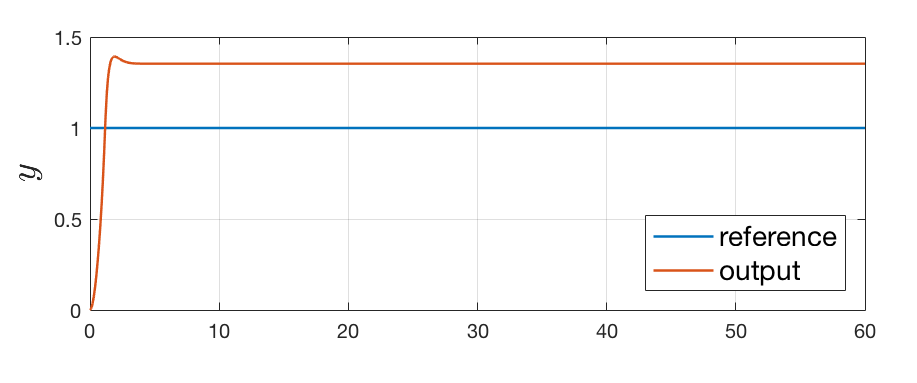
\includegraphics[scale=0.7]{NonLinearControl/images/FL_tracking.png}
    \caption{Tracking error in presence of uncertainties (FL)}
    \label{fig:enter-label}
\end{figure}

\noindent
We have the same setting as Feedback linearization, the (nonlinear) system is in the form: 
\begin{equation}
    \begin{aligned}
        &\dot{x}=f(x)+g(x)u\\
        &y=h(x)
    \end{aligned}
\end{equation}
which can be lead to the \textit{normal form} that distinguishes: the external dynamics described by the state transformation $x\rightarrow \mu$ and the internal dynamics described by $\dot{\psi}$ assumed to be locally asymptotically stable.\\
Suppose now that the system output $y(t)$ is required to track a reference signal $r(t)$. In a way similar to the FL, we define the \textit{tracking error} as $\Tilde{y}\doteq  r-y$. Even in this case we want to make it "small" and force it to converge to zero.\\

Now a set of definitions are given as ingredient to introduce the \textbf{Sliding mode control} method.\\

\hspace*{-5mm}
\begin{tikzpicture}
\node [mybox] (box){%
    \begin{minipage}{.96\textwidth}     %Larghezza del box
    \textbf{Definition (Sliding surface)} The \textbf{sliding surface} is $$S(t)\doteq\{x\in \mathbb{R}^n : \textbf{s}(x, t)=0 \}$$ where the function $\textbf{s}:\mathbb{R}^{n+1}\rightarrow\mathbb{R}$ is defined as follows
    \begin{align*}
        \textbf{s}(x,t)&=\Tilde{y}^{(\gamma-1)}+k_\gamma \Tilde{y}^{(\gamma-2)}+...+k_2\Tilde{y}=\\
        &=\Tilde{\mu}_\gamma+k_\gamma \ \Tilde{\mu}_{\gamma-1}+...+k_2 \ \Tilde{\mu}_1   
    \end{align*}
    
    the coefficients $k_i\in \mathbb{R}$ are chosen so that the roots of the polynomial ${P(\lambda)=\lambda^{\gamma-1}+k_\gamma\lambda^{\gamma-2}+...+k_2}$ have \textbf{negative real part}.
    \end{minipage}
};
\end{tikzpicture}%

\section{Behaviour on the sliding surface}
{\color{red} \textbf{Property 1}}: If the trajectory of the system is confined to the sliding surface, then the tracking error $\Tilde{y}\rightarrow 0$, in a way that depends on the root of $P(\lambda)$.\\

Due to the fact that the system has a nice behaviour if the \textbf{Property 1} is verified, we would like to find a control law such that the sliding surface $S$ could be: 
\begin{itemize}
    \item \textbf{\underline{Invariant}}: if the trajectory is on S, it remains on it; that is $x(\tau)\in S(\tau) \Rightarrow x(t)\in S(t), \forall t \ge \tau$; 
    \item \textbf{\underline{Attractive}}: if the trajectory is outside of the sliding surface $S$, it is forced to move toward it in a finite time.
\end{itemize}

The motion of the system on this surface is called \textbf{sliding mode}, from this fact is derived the name \textbf{Sliding mode control}.

\begin{figure}[h]
    \centering
    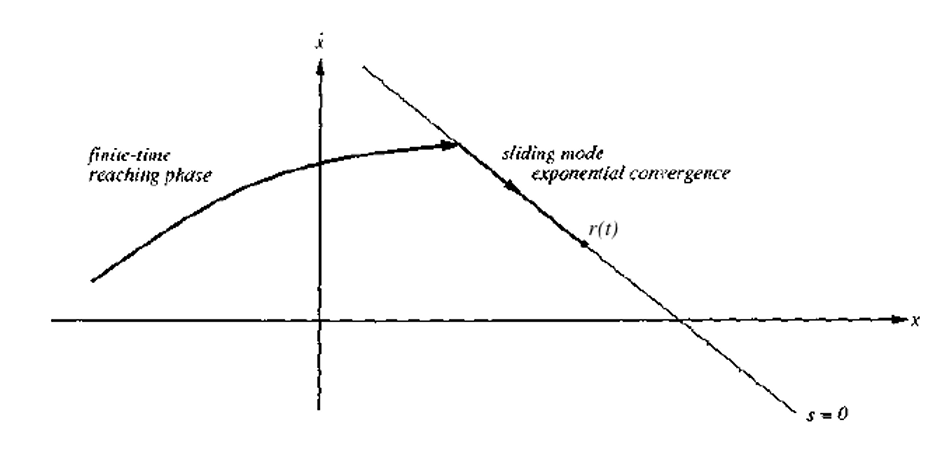
\includegraphics[scale=0.7]{NonLinearControl/images/SMC.png}
    \label{fig:enter-label}
\end{figure}

\subsection{Invariance of the Sliding surface}
If in a certain time $\tau$ the trajectory of the system lie on the sliding surface, then as defined before $x(\tau)\in S \Rightarrow \textbf{s}(x(\tau), \tau)=0$. In order to guarantee the invariance of the surface we have to put $\dot{\textbf{s}}=0 \quad \forall t$.\\
\begin{align*}
&\dot{\textbf{s}}=\Tilde{y}^{(\gamma)}+k_\gamma \Tilde{y}^{(\gamma-1)}+...+k_2\dot{\Tilde{y}}=0 \Longleftrightarrow r^{(\gamma)}-a(x)-b(x)u+k_\gamma y^{(\gamma-1)}+...+k_2 \dot{\Tilde{y}}=0\\
    &
\end{align*}
where we used $\Tilde{y}^{(\gamma)}=r^{(\gamma)}-y^{(\gamma)}=
r^{(\gamma)}-a(x)-b(x)u$. \\
Solving the equation for $u$ we obtain the following control law
\begin{equation}
    u_s=\frac{1}{b(x)}\bigg(r^{(\gamma)}-a(x)+k_\gamma \Tilde{y}^{(\gamma-1)}+...+k_2 \dot{\Tilde{y}} \bigg)
\end{equation}
\noindent
{\color{red} \textbf{Property 2}}: using this law, the sliding surface is an \underline{invariant set}. 

\subsection{Attractiveness of the Sliding surface}
Suppose that at a certain instant $\tau$ the trajectory is not on the sliding surface. We would like to bring it toward $S(t)$ in a finite time. \\
The introduction of a discontinuous term to $u_s$ make $S$ attractive. Then, the \textit{complete control law} is the following, let $k_1>0$: 
$$ u_s=\frac{1}{b(x)}\bigg(r^{(\gamma)}-a(x)+k_\gamma \Tilde{y}^{(\gamma-1)}+...+k_2 \dot{\Tilde{y}} +k_1 \text{sign}(\textbf{s}(x,t))\bigg)$$
The motivation of adding a discontinuous term is the fact that in this way the derivative of the sliding function 
\begin{align}
    \dot{\textbf{s}}(x,t)&= r^{(\gamma)}-a(x)-b(x)u+k_\gamma \Tilde{y}^{(\gamma-1)}+...+k_2 \dot{\Tilde{y}}=\\
    &=-k_1\text{sign}(\textbf{s}(x,t)).
\end{align}

\noindent
{\color{red}\textbf{Property 3}}:  $\textbf{s}(x,t) \ \dot{\textbf{s}}(x,t)<0,\quad \forall x,t$, which implies that $S(t)$ is attractive (the sliding function \textbf{s} converges to zero in finite time). In particular: 
\begin{itemize}
    \item $\textbf{s}(x,\tau)>0 \Rightarrow \dot{\textbf{s}}=-k_1 $
    \begin{align*}
        &\int_{\tau}^{t} \dot{\textbf{s}}\ dt = \int_{\tau}^{t} -k_1\ dt 
        \Longleftrightarrow \textbf{s}(t)-\textbf{s}(\tau)=-k_1(t-\tau) \Longleftrightarrow
        &\textbf{s}(t)=\textbf{s}(\tau)-k_1(t-\tau)
    \end{align*}
    \item $\textbf{s}(x,\tau)<0 \Rightarrow \dot{\textbf{s}}=k_1$
    \begin{align*}
       &\int_{\tau}^{t} \dot{\textbf{s}}\ dt = \int_{\tau}^{t} k_1\ dt 
        \Longleftrightarrow \textbf{s}(t)-\textbf{s}(\tau)=k_1(t-\tau) \Longleftrightarrow
        &\textbf{s}(t)=\textbf{s}(\tau)+k_1(t-\tau)
    \end{align*}
\end{itemize}

\noindent
In both cases, $\textbf{s}(t)\rightarrow 0$ in finite time $\Rightarrow$ $x(t)\rightarrow S(t)$ in finite time applying the input with discontinuous term.

\subsection{Chattering}
The presence of the discontinuous term may cause a phenomenon called \textbf{chattering} which consists of high frequency oscillations around the sliding surface. To avoid this problem we can use a \textbf{sigmoid function} $\sigma(\eta \textbf{s})$, where $\eta$ is a design parameter which defines the slope of the sigmoid itself. The function $\sigma(\eta\textbf{s})=\tanh{(\eta\textbf{s})}$ is a typical choice. The control law becomes:\\

\begin{figure}[h]
    \centering
    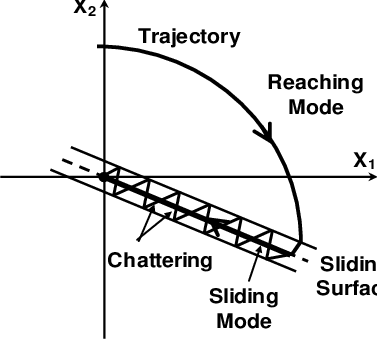
\includegraphics[scale=0.7]{NonLinearControl/images/Chattering.png}
    \caption{Chattering phenomenon}
    \label{fig:enter-label}
\end{figure}

\hspace*{-5mm}
\begin{tikzpicture}
\node [mybox] (box){%
    \begin{minipage}{.96\textwidth}     %Larghezza del box
    $$u_s=\frac{1}{b(x)}\bigg(r^{(\gamma)}-a(x)+k_\gamma \ \Tilde{y}^{(\gamma-1)}+...+k_2 \ \dot{\Tilde{y}} +k_1 \sigma(\eta\textbf{s})\bigg) $$
    \end{minipage}
};
\end{tikzpicture}%
\begin{figure}[h]
    \centering
    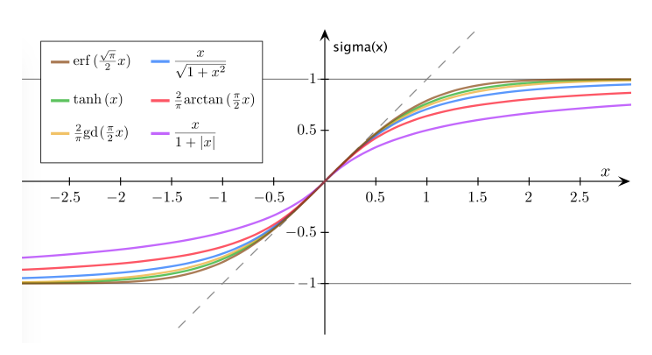
\includegraphics{NonLinearControl/images/sigmoids.png}
    \caption{Alternatives to sign(\textbf{s})}
    \label{fig:enter-label}
\end{figure}

\section{Comparison with feedback linearization}
The two approaches of \textbf{Feedback linearization} and \textbf{Sliding mode control} have a common general control law given by: 
$$u=\frac{1}{L_gL_f^{\gamma-1}h(x)}(-L_f^{\gamma}h(x)+v)=\frac{1}{b(x)}(-a(x)+v)$$
The techniques have the $v$ which differs of a term. More specifically, let $\Tilde{\mu}_i=r^{(i)}-y^{(i)}=\tilde{y}^{(i)}$
\begin{itemize}
    \item In the feedback linearization: $v=r^{(\gamma)}+k_\gamma \ \Tilde{\mu}_\gamma+...+k_1 \ \Tilde{\mu}_1$
    \item In the sliding mode control: $v=r^{(\gamma)}+k_\gamma \ \Tilde{\mu}_\gamma+...+k_1 \ \sigma(\eta\textbf{s})$
\end{itemize}
The term which is different increases the robustness of the controller.

\section{Control Scheme}
Even the general control scheme is quite similar to the feedback linearization, the only difference is that instead of the linear controller there is a block that provided $r^{(\gamma)}$ and $\Tilde{\mu}$ gives the sliding control law $v=r^{(\gamma)}+k_\gamma \ \Tilde{\mu}_\gamma+...+k_1 \ \sigma(\eta\textbf{s})$

\begin{figure}[h]
    \centering
    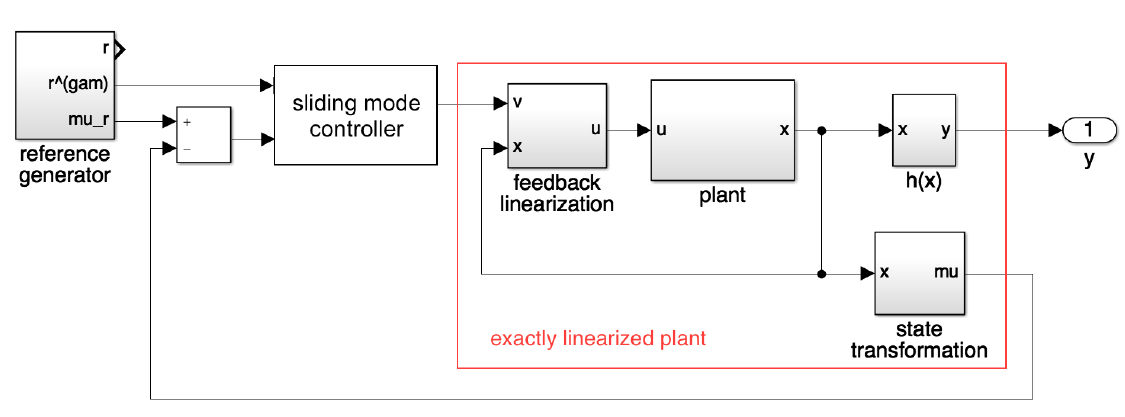
\includegraphics[scale=0.6]{NonLinearControl/images/SMC_ControlScheme.png}
    \caption{Sliding control mode general control scheme}
    \label{fig:enter-label}
\end{figure}



\section{Robustness properties}
Now we consider the case when the system to control in \underline{not exactly known}. In normal form we can describe the fact in this way: 
{\color{red}$$y^{(\gamma)}=a(x)+\Delta a(x) +b(x)u$$}

Where $\Delta a(x)$ is a smooth function of $\mathbb{R}^{n_x}$ but it is \underline{unknown}, moreover we know that ${\lVert \Delta a(x) \rVert \le \bar{\Delta}, \ \forall x \in \mathbb{R}^n}$. In this way the time derivative of the sliding function is: 
$$ \dot{\textbf{s}}(x, t)=-\Delta a(x)-k_1 \ \sigma(\eta\textbf{s})$$
In the context of uncertainty in the model of the plant it holds that:\\

\noindent
{\color{red}\textbf{Property 4}}: If $k_1>\bar{\Delta}$, then the sliding surface is attractive. \\

The figure below shows the \textit{step response} for a sliding mode controlled system in which uncertainty appears. In particular for control design we use the approximated $\hat{\rho}(x_1)$, while the plant has the real nonlinearity which is a piece-wise function $\rho(x_1)$. The tracking error is smaller than the case of a controller built by using the feedback linearization technique.

\begin{figure}[h]
    \centering
    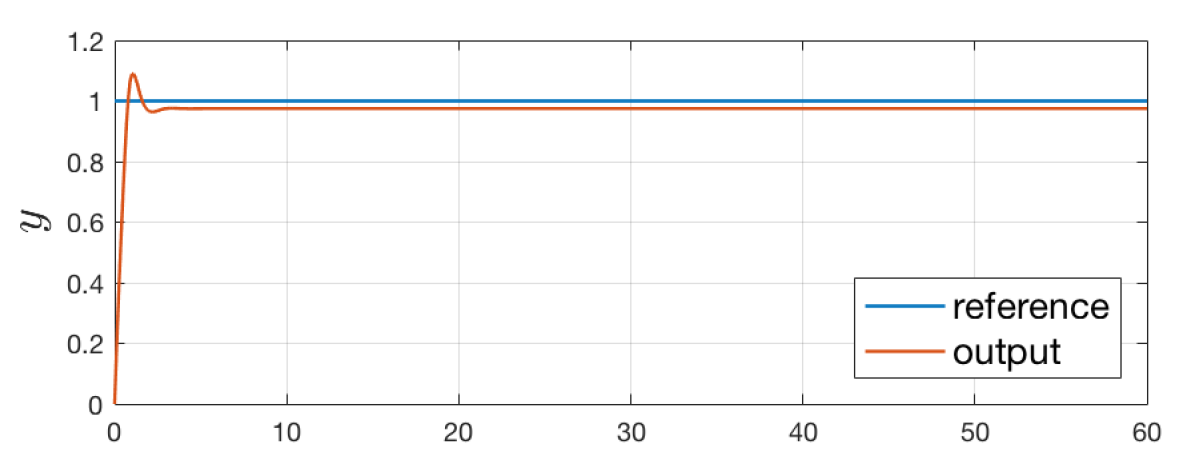
\includegraphics[scale=0.7]{NonLinearControl/images/SMC_Tracking.png}
    \caption{Step response: sliding mode controller}
    \label{fig:enter-label}
\end{figure}

\section{Guidelines for the choice of the SM parameters}
\begin{itemize}
    \item The parameters $k_i, \ i=\gamma, \gamma-1, ..., 2$ are the coefficients  of the polynomial $P(\lambda)$. Useful indications can be:
    \begin{itemize}
        \item All the roots must have negative real part;
        \item The speed of convergence is linked to the value of the $k_i$
        \item At the same time they cannot be too much large this would result in too high command activity
    \end{itemize}
    \item The parameter $k_1>0$ allows us to \textbf{increase the closed-loop robustness}: The larger is $k_1$ the more robust is the closed-loop system, but too large value of this parameter results in significant \textbf{chattering phenomena} and \textbf{high command activity};
    \item Using the hyperbolic tangent function instead of sign requires to choose the additional parameter $\eta$. A large value of $\eta$ can be taken initially so that $\tanh \simeq \text{sign}$, then $\eta$ can be gradually reduced in order to reduce the chattering pheonomena without compromising too much \textbf{performance} and \textbf{robustness}.
    
\end{itemize}

\section{Discussion}
Sliding mode control is a technique which has strong theoretical behaviuor, is robust to model uncertainties and disturbances of a certain type for the mentioned reasons this method give \textbf{high control performances}. \\
On the other hand, as usual, there are some \textbf{drawbacks}:
\begin{itemize}
    \item The model is assumed to be affine in $u$, it cannot have whatever structure; 
    \item When the internal dynamics is stable everything works well, otherwise we can't approach the control problem; sometimes it is sufficient to change the output to make the same problem easier and so tractable; 
    \item in general there is an \textbf{high command activity}.
\end{itemize}
Possible extensions of the concepts exposed here are possible for systems which have multiple input and multiple output (MIMO).
